\documentclass[conference,10pt,compsocconf]{IEEEtran}

% *** CITATION PACKAGES ***
%
\usepackage{cite}
% cite.sty was written by Donald Arseneau
% V1.6 and later of IEEEtran pre-defines the format of the cite.sty package
% \cite{} output to follow that of IEEE. Loading the cite package will
% result in citation numbers being automatically sorted and properly
% "compressed/ranged". e.g., [1], [9], [2], [7], [5], [6] without using
% cite.sty will become [1], [2], [5]--[7], [9] using cite.sty. cite.sty's
% \cite will automatically add leading space, if needed. Use cite.sty's
% noadjust option (cite.sty V3.8 and later) if you want to turn this off.
% cite.sty is already installed on most LaTeX systems. Be sure and use
% version 4.0 (2003-05-27) and later if using hyperref.sty. cite.sty does
% not currently provide for hyperlinked citations.
% The latest version can be obtained at:
% http://www.ctan.org/tex-archive/macros/latex/contrib/cite/
% The documentation is contained in the cite.sty file itself.
%
\usepackage{setspace}
\usepackage{wrapfig}
\usepackage[usenames, dvipsnames]{color}
\usepackage{balance}

%\usepackage[pdftex]{graphicx}
\usepackage{graphicx}
% declare the path(s) where your graphic files are
\graphicspath{{./}{./figs}}
% and their extensions so you won't have to specify these with
% every instance of \includegraphics
\DeclareGraphicsExtensions{.pdf,.jpeg,.png}

% *** SUBFIGURE PACKAGES ***
\usepackage[tight,footnotesize]{subfigure}
% \usepackage{subfigure}
% subfigure.sty was written by Steven Douglas Cochran. This package makes it
% easy to put subfigures in your figures. e.g., "Figure 1a and 1b". For IEEE
% work, it is a good idea to load it with the tight package option to reduce
% the amount of white space around the subfigures. subfigure.sty is already
% installed on most LaTeX systems. The latest version and documentation can
% be obtained at:
% http://www.ctan.org/tex-archive/obsolete/macros/latex/contrib/subfigure/
% subfigure.sty has been superceeded by subfig.sty.

%\usepackage[caption=false]{caption}
%\usepackage[font=footnotesize]{subfig}
% subfig.sty, also written by Steven Douglas Cochran, is the modern
% replacement for subfigure.sty. However, subfig.sty requires and
% automatically loads Axel Sommerfeldt's caption.sty which will override
% IEEEtran.cls handling of captions and this will result in nonIEEE style
% figure/table captions. To prevent this problem, be sure and preload
% caption.sty with its "caption=false" package option. This is will preserve
% IEEEtran.cls handing of captions. Version 1.3 (2005/06/28) and later
% (recommended due to many improvements over 1.2) of subfig.sty supports
% the caption=false option directly:
%\usepackage[caption=false,font=footnotesize]{subfig}
%
% The latest version and documentation can be obtained at:
% http://www.ctan.org/tex-archive/macros/latex/contrib/subfig/
% The latest version and documentation of caption.sty can be obtained at:
% http://www.ctan.org/tex-archive/macros/latex/contrib/caption/

% *** PDF, URL AND HYPERLINK PACKAGES ***
%
\usepackage{url}
% url.sty was written by Donald Arseneau. It provides better support for
% handling and breaking URLs. url.sty is already installed on most LaTeX
% systems. The latest version can be obtained at:
% http://www.ctan.org/tex-archive/macros/latex/contrib/misc/
% Read the url.sty source comments for usage information. Basically,
% \url{my_url_here}.

% *** Do not adjust lengths that control margins, column widths, etc. ***
% *** Do not use packages that alter fonts (such as pslatex).         ***
% There should be no need to do such things with IEEEtran.cls V1.6 and later.
% (Unless specifically asked to do so by the journal or conference you plan
% to submit to, of course. )

\usepackage{draftwatermark}

\newcommand{\assign}[1]{\textcolor{red}{(#1)}}
\newcommand{\todo}[1]{\textcolor{Orange}{TODO: #1}}

\begin{document}
\title{HPC I/O Ecosystem Instrumentation: Insights from correlating data}

\maketitle

\begin{abstract}

I/O efficiency is essential to productivity in scientific computing,
especially as most scientific domains become more data-intensive and
new large-scale computing platforms incorporate more complex storage
hierarchies.  A variety of instrumentation and analysis tools have been
utilized to great effect to help understand and optimize specific aspects of
HPC I/O, such as application access patterns, storage device traffic, and
distributed file system configurations.  However, analyzing individual services in the
I/O ecosystem in isolation fails to provide insight into the most important
questions: how do the I/O components interact, what \emph{combinations}
of optimizations across the stack are most effective, and what are the
underlying causes and effects of I/O performance problems?

In this work we explore the potential for holistic I/O characterization
by combining I/O instrumentation data from multiple sources to obtain
insights that were previously unobtainable. We describe a methodology that
incorporates file system instrumenatation, application instrumentation,
health monitoring, and formalized periodic regression benchmarking as
the foundation of portable I/O instrumentation, and then demonstrate
its applicability, portability, and inobtrusiveness by deploying that
methodology in production on two distinct leadership-class computing
platforms. Based on our \todo{some time period} study we observe
\todo{some outcome}.

\end{abstract}

\section{Introduction \assign{Phil}}

\emph{From Rob}: I think a component of the story is that when we approach these problems, there are a few challenges:
\begin{enumerate}
\item increasing number of interoperating components (in this case, additional
BB and DVS and so forth)
\item different components have different "views" on I/O, different levels of
monitoring, some of which aren't practical in production
\item no current framework for integration, lots of expert knowledge to
construct the story of what happened and how to fix.
\end{enumerate}
Cite something to get bibtex working for now~\cite{carns200924}.

The primary contributions of this work are as follows:

\begin{itemize}
\item A proposed model for holistic instrumentation of I/O subsystems,
including identification of the key roles that individual data streams play
\item An implementation of this model on two large-scale, diverse HPC
platforms
\item A demonstration of the types of insights that can be gleaned from this
approach based on a case study of N scientific applications executed in a
production environment
\end{itemize}

\section{Instrumentation methods}

Brief description of tools that we are using.
\todo{overview diagram here?}

\subsection{Darshan \assign{Shane}}

\subsection{LMT \assign{Glenn}}

The Lustre Monitoring Tool (LMT) is a framework that collects Lustre-specific
counters from \texttt{/proc/fs/lustre} on each Lustre OSS and MDS and presents
them to external consumers via a MySQL database.  NERSC Edison, NERSC Cori, and
ALCF Theta all implement LMT as a part of the Cray Sonexion Lustre platform
\cite{Keopp2014}, and we built upon the pyLMT framework developed at NERSC
\cite{Uselton2009} to preserve server-side metrics during benchmark runs across
all file systems evaluated.  These metrics include bytes read and written, CPU
load averages, and metadata operation rates on a per-server basis at
five-second intervals.

\subsection{mmpmon \assign{Phil}}

Pull in Zach as needed.

\subsection{health monitoring \assign{Glenn and Phil}}

Do capacity monitoring and failover monitoring for both Lustre and GPFS.  The
tools themselves are probably very simple, we should focus on how you go
about extracting this information.

\section{Platforms and workloads}

We employ our methodology on two platforms:

\begin{itemize}
\item \textbf{Cori} \assign{Glenn}
\item \textbf{Mira} \assign{Phil}
\end{itemize}

We selected 4 represenative application workloads for periodic regression
benchmarking:

\begin{itemize}
\item \textbf{HACC} \assign{Shane}
\item \textbf{VPIC} \assign{Suren} \cite{Bowers2008}
\item \textbf{BDCATS} \assign{Suren} The BD-CATS-IO benchmark emulates the I/O
pattern of the BD-CATS clustering system\cite{Patwary2015}, and it represents
one of the analyses that is performed on the output of VPIC's particle files.
For this study, we emulate the I/O workload of a clustering both partical
positions and momenta in three dimensions.  This amounts to 75\% of the data
contained in the HDF5 file (generated by the VPIC-IO benchmark) being read.
\item \textbf{IOR} \assign{Shane}
\end{itemize}

\todo{Describe how we are scheduling these jobs to run.} \assign{Glenn}

\todo{Here or in evaluation, describe how we sized the jobs for each
platform.  See mailing list discussion Jan27-Feb6.  Mira has fixed ratio of
ions to compute nodes, Cori does not, leads to different characteristics.  In
either case goal is to exercise file system as much as we can within job
sizes that will get through queue in daily cadence.}

\subsection{Mira benchmark configuration}

Mira's I/O architecture is fundamentally different from that of the Cray
systems at NERSC, with fixed-size partitions of compute nodes connected to
a single I/O node that forwards application I/O requests to the SAN.
Saturating the I/O bandwidth of the underlying storage servers requires the
use of many I/O nodes, meaning that peak storage bandwidth can only be
attained using a large portion of the system's available compute nodes.
Running daily I/O benchmarks that span a large portion of Mira's compute
nodes is impractical due to the lengthy queue times of capability jobs and
the obvious objection system administrators would have to this practice.

For these reasons, we decided to use 1,024 Mira compute nodes (i.e., a single
rack), a partition size that should be small enough to move quickly through
scheduler queues, but large enough to exercise an adequate portion of the
storage system. We use 16 processes per node, resulting in a total of 16,384
processes executing each benchmark. The benchmark workloads were configured
to use enough I/O volume to drive the storage system for 1--2 minutes.
Full benchmark configurations for Mira are given below in
Table~\ref{tab:mira-bench-config}.

\begin{table*}[h]
\centering
\begin{tabular}{|c|c|c|c|c|c|c|}
\hline
benchmark & I/O motif & node count & proc count & I/O volume & I/O b/w (GiB/s) & I/O time (s) \\
\hline
IOR & MPI-IO; shared-file; write & 1,024 & 16,384 & 1 TiB & 9.7 & 106 \\
\hline
IOR & MPI-IO; shared-file; read & 1,024 & 16,384 & 1 TiB & 8.4 & 125 \\
\hline
IOR & POSIX; file-per-process; write & 1,024 & 16,384 & 1 TiB & 13.5 & 76 \\
\hline
IOR & POSIX; file-per-process; read & 1,024 & 16,384 & 1 TiB & 18.5 & 56 \\
\hline
HACC-IO & GLEAN; file-per-process; write & 1,024 & 16,384 & ~1.5 TiB & 1.6 & 900 \\
\hline
HACC-IO & GLEAN; file-per-process; read & 1,024 & 16,384 & ~1.5 TiB & 17.2 & 90 \\
\hline
VPIC-IO & pHDF5; shared file; write & 1,024 & 16,384 & ~1 TiB & 16.4 & 62.4 \\
\hline
BDCATS-IO & pHDF5; shared file; read & 1,024 & 16,384 & ~768 GiB & 12.2 & 62.8 \\
\hline
\end{tabular}
\caption{Caption.}
\label{tab:mira-bench-config}
\end{table*}

\section{Evaluation}

\todo{Fill this section in based on what we observe}

\begin{figure}[t]
\centering
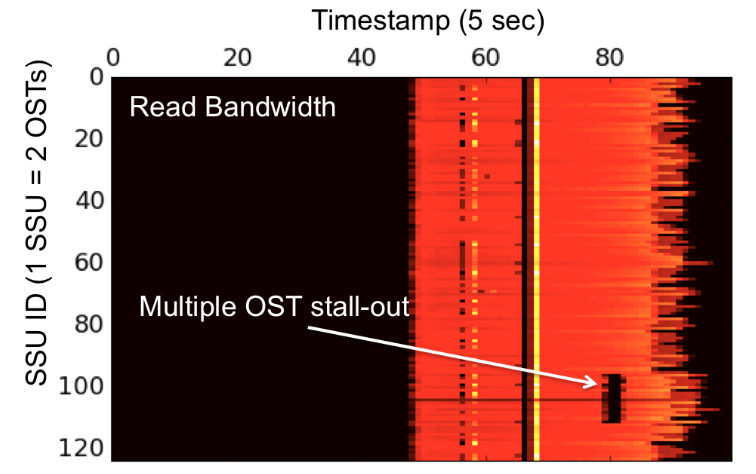
\includegraphics[width=0.8\columnwidth]{figs/example.png}
%\vspace{-.07in}
\caption{Example figure showing server-side read bandwidth with an artifact
caused by a Lustre server problem.}
\label{fig:example}
\vspace{-.1in}
\end{figure}

\begin{figure}[t]
\centering
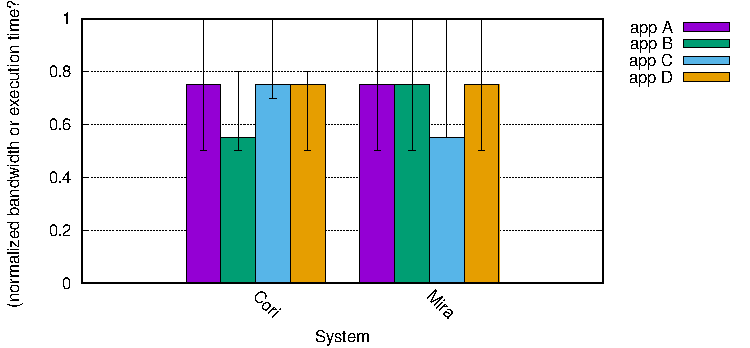
\includegraphics[width=0.8\columnwidth]{figs/example-bar-var.pdf}
%\vspace{-.07in}
\caption{Example of how to illustrate difference in relative performance of
benchmarks across platforms.  Whiskers for either confidence intervals or
min/max, bars for median across samples.  Expect shape of clusters (i.e.
which benchmark performs best) to differ.}
\label{fig:example-bar-var}
\vspace{-.1in}
\end{figure}

\begin{itemize}
\item Sometimes metadata operations are slow (e.g., file-per-process I/O)
    \begin{itemize}
    \item Show Darshan logs showing high metadata time
    \item Show LMT MDT logs showing high background metadata or CPU rate
    \item Show GPFS NSD metadata loads?  Can we do this?
    \end{itemize}
\item Sometimes hardware goes bad
    \begin{itemize}
    \item Show Darshan logs showing bad performance at the POSIX layer (i.e., not the
    application's fault)
    \item Show Lustre OSTs that stall out, e.g, Figure~\ref{fig:example}
    \item Show slow Lustre OSTs due to failover/oversubscription (a la Darshan 3 paper)
    \item Show poorly performing GPFS NSDs
    \end{itemize}
\item Sometimes there is interference from other applications
    \begin{itemize}
    \item Show Darshan logs showing bad performance at the POSIX layer (i.e., not the
    application's fault)
    \item Show jobs with and without background LMT load
    \item Show jobs with and without background mmpmon load
    \end{itemize}
\item Sometimes tuning strategies differ across platforms
    \begin{itemize}
    \item contrast which benchmark performs best on each platform
    \item dig into why
    \item See example of how we might show this in Figure~\ref{fig:example-bar-var}
    \end{itemize}
\end{itemize}

\subsection{Discussion}

\begin{itemize}
\item Make statements about how often bad I/O performance can be attributed to each
of the different causes we categorized--that is, break down what the most
common sources of performance degradation are
\item Make statements about how susceptible different file systems are to these bad
I/O performance root causes to stir up controversy (GPFS is better/worse than
Lustre when facing problem X)
\item Propose that holistic I/O monitoring can provide a feedback loop for
coscheduling (to hit some buzzwords)
\end{itemize}

\section{Related work}

\assign{Phil} \todo{include SIOX, Xiaosong Ma's work}

\section{Conclusions}

\todo{It would be great if there were some tangible artifacts from this work.
Possible examples:}
\begin{itemize}
\item open repo for benchmark configs and cron jobs so others can replicate
performance regression testing
\item anonymized data collected in study
\item new data collection tools (LMT monitoring, Lustre failover monitoring,
mmpmon monitoring, etc.)
\end{itemize}

\section{TEMPORARY: TECHNICAL TASKS}

Assumption: assignments here and in preceding text are tentative, and really
just guess at someone who can keep tabs on that activity.  Can re-assign,
delegate, pull in more people, etc.

Assumption: although the paper as outlined will focus on Cori and Mira, we
should actually try to do these things across Theta and Edison as well.  Four
total platforms, and we'll see which ones are most viable for study in paper.

To do:
\begin{itemize}
\item create git repository to store benchmarks, config files, job scripts,
and cron configs for our set of benchmarks \assign{Shane}
\begin{itemize}
\item repo status: includes build scripts for hacc-io, bdcats, vpic, and ior
\item everything works at nersc, currently testing in 96 node runs on Cori
and Edison
\item todo: review configurations, get ALCF configs working, settle on
size/duration
\end{itemize}

% other benchmarks to consider later: chombo and newer version of hacc-io
% with hdf support

\item make sure that mmpmon monitoring gets deployed on Mira \assign{Phil and
Kevin}
\begin{itemize}
\item timeline: currently running on Vesta, will be running on Cetus this
Monday, will be running on Mira 2 weeks later if things look good
\item long term plan to do same thing on Theta DVS nodes
\end{itemize}

\item coordinate LMT monitoring methods on Theta \assign{Glenn and Kevin}
\begin{itemize}
\item Meeting about this on Tuesday
\end{itemize}

\item enable cron jobs to run periodic jobs on ALCF machines \assign{Shane}
\begin{itemize}
\item Kevin working on this for Mira using Jenkins
\item on Theta we will need to use cron with flock -n wrapper
\end{itemize}

\item enable cron jobs to run periodic jobs on NERSC machines \assign{Glenn}
\begin{itemize}
\item probably won't fit in backfill as is, can work on reducing time, maybe
consider killalble queue too
\item Glenn has been getting 4 hour runs through queue so far without much
trouble using 96 nodes
\item Glenn: has a master script for this already, gradually hardening, will
add to git repo
\item For paper: measure saturation percentage of scripts and give rationale
for jobs of different sizes on different machines being comparable
\item remember to plot in relative rather than absolute times in paper where
we can, don't want people to get distracted by head to head comparison
\end{itemize}

\item create and enable cron jobs to check Lustre failover status and server
capacity
\begin{itemize}
\item Glenn: already collecting this data at NERSC now
\end{itemize}

\item create and enable cron jobs to check GPFS failover status and server
capacity
\begin{itemize}
\item plan to use Zach's periodic df monitoring data
\item for failover we will have to look at logs, they are doing some
automation already
\end{itemize}

\item start browsing existing HACC-IO data collected by Glenn to think about
how to plot it, how to dig into details, etc. \assign{ALL}
    
\item contrast benchmark performance across platforms once we have stable
daily data \assign{William and Suren}
\end{itemize}

Timeline:
\begin{itemize}
\item Start running periodic (daily) jobs by mid-January
\item writing up text based on results by mid-February
\end{itemize}

Stretch goals:
\begin{itemize}
\item additional instrumentation sources
\item more contributions from analysis framework perspective (i.e.,
leveraging work from William's paper) 
\item deploy on more platforms (either additional ALCF or NERSC systems, or
reach out to another facility like Blue Waters)
\end{itemize}

\bibliographystyle{IEEEtran}
\bibliography{REFERENCES}


\appendix

\section{Artifact Description}

Consider adding material here per guidance at
\url{http://sc17.supercomputing.org/2017/02/07/submitting-a-technical-paper-to-sc17-participate-in-the-sc17-reproducibility-initiative/}.


\end{document}
